%%%%%%%%%%%%%%%%%%%%%%%%%%%%%%%%%%%%%%%%%%%%%%%%%%%%%%%%%%%%%%%%%%%%%%%%
%                                                                      %
%     File: Thesis_Background.tex                                      %
%     Tex Master: Thesis.tex                                           %
%                                                                      %
%     Author: Andre C. Marta                                           %
%     Last modified :  4 Mar 2024                                      %
%                                                                      %
%%%%%%%%%%%%%%%%%%%%%%%%%%%%%%%%%%%%%%%%%%%%%%%%%%%%%%%%%%%%%%%%%%%%%%%%


\chapter{Background}
\label{chapter:background}

This chapter presents the theoretical and modelling foundations of the work, including an overview of the underlying concepts, the mathematical models of the system components, and the formulation of the control framework.

It is important to clarify the current scope of the work. Although the complete system comprises three coupled agents, a \gls{uav}, a \gls{usv}, and a tether, the \gls{usv} is not yet modelled or considered in the present stage. The focus is placed on a tethered \gls{uav} subsystem to enable the step-by-step development and validation of the proposed approach. The inclusion of the surface vessel within the same unified framework will be addressed in the full dissertation.


%%%%%%%%%%%%%%%%%%%%%%%%%%%%%%%%%%%%%%%%%%%%%%%%%%%%%%%%%%%%%%%%%%%%%%%%%%%%%

% MODELS

%%%%%%%%%%%%%%%%%%%%%%%%%%%%%%%%%%%%%%%%%%%%%%%%%%%%%%%%%%%%%%%%%%%%%%%%%%%%%
\section{System Modelling}
\label{sec:theoretical_model_1}

\subsection{Modelling Principles}
\label{subsec:modelling_identification}

The objective of the system modelling in this work is to provide an accurate and control-oriented representation of the system dynamics, serving as the foundation for the motion control framework developed in subsequent sections. The adopted models aim to achieve a balance between physical accuracy and computational tractability, ensuring real-time feasibility while capturing the dominant dynamic effects governing the system behaviour \citep{modeling_Silva}.

Given the strong coupling introduced by the tether and the need for explicit dynamic consistency, the modelling approach initially follows a white-box methodology based on first-principles kinematic and dynamic formulations of the individual agents. This provides physically interpretable models with a clear structure for control design \citep{slotineAppliedNonlinearControl1991}. At later stages of the research, the framework may be extended towards a grey-box formulation by incorporating parameter estimation or simple data-driven refinements from experimental or simulated data to capture residual effects not fully represented in the physical model \citep{system_identification_Ljung,tangirala2013principles,houModelbasedControlDatadriven2013}.

In general, the dynamic behaviour of a nonlinear control system can be expressed in continuous-time state-space form as \citep{slotineAppliedNonlinearControl1991,rawlingsModelPredictiveControl2020}
\begin{equation}
\dot{x} = f(x, u, t) + w,
\end{equation}
where \(x \in \mathbb{R}^n\) denotes the system state vector, \(u \in \mathbb{R}^m\) the control input vector, and \(w \in \mathbb{R}^n\) represents model uncertainties or external disturbances. This compact representation provides a unified mathematical structure for describing the system dynamics and forms the basis for the control formulation developed in later sections.


\subsection{Dynamic Modelling of the tethered UAV Subsystem}
\subsubsection{Reference Frames and Notation}

In this work, the \gls{uav} is modelled using a geometric formulation based on position vectors and rotation matrices \citep{slotineAppliedNonlinearControl1991,beardSmallUnmannedAircraft2012}.
 Linear and angular velocities \((v, \omega)\) are expressed in a body-fixed reference frame, while positions and trajectories are expressed in an inertial reference frame.

To describe the motion of the aerial vehicle relative to the Earth and its own orientation, two coordinate frames are defined, as illustrated in Fig.~\ref{fig:reference_frames}:
\begin{itemize}
    \item An inertial reference frame \(\{\mathcal{I}\}\), defined under a flat-Earth assumption.
    \item A body-fixed reference frame \(\{\mathcal{B}\}\), rigidly attached to the \gls{uav}.
\end{itemize}

The configuration of the \gls{uav} is described by the pair \((p, R)\), where:
\begin{itemize}
    \item \(p \in \mathbb{R}^3\) denotes the position of the origin of \(\{\mathcal{B}\}\) expressed in \(\{\mathcal{I}\}\).
    \item \(R \in SO(3)\) represents the rotation matrix that transforms a vector expressed in the body-fixed frame \(\{\mathcal{B}\}\) into its representation in the inertial frame \(\{\mathcal{I}\}\).
\end{itemize}

\begin{figure}[H]
    \centering
    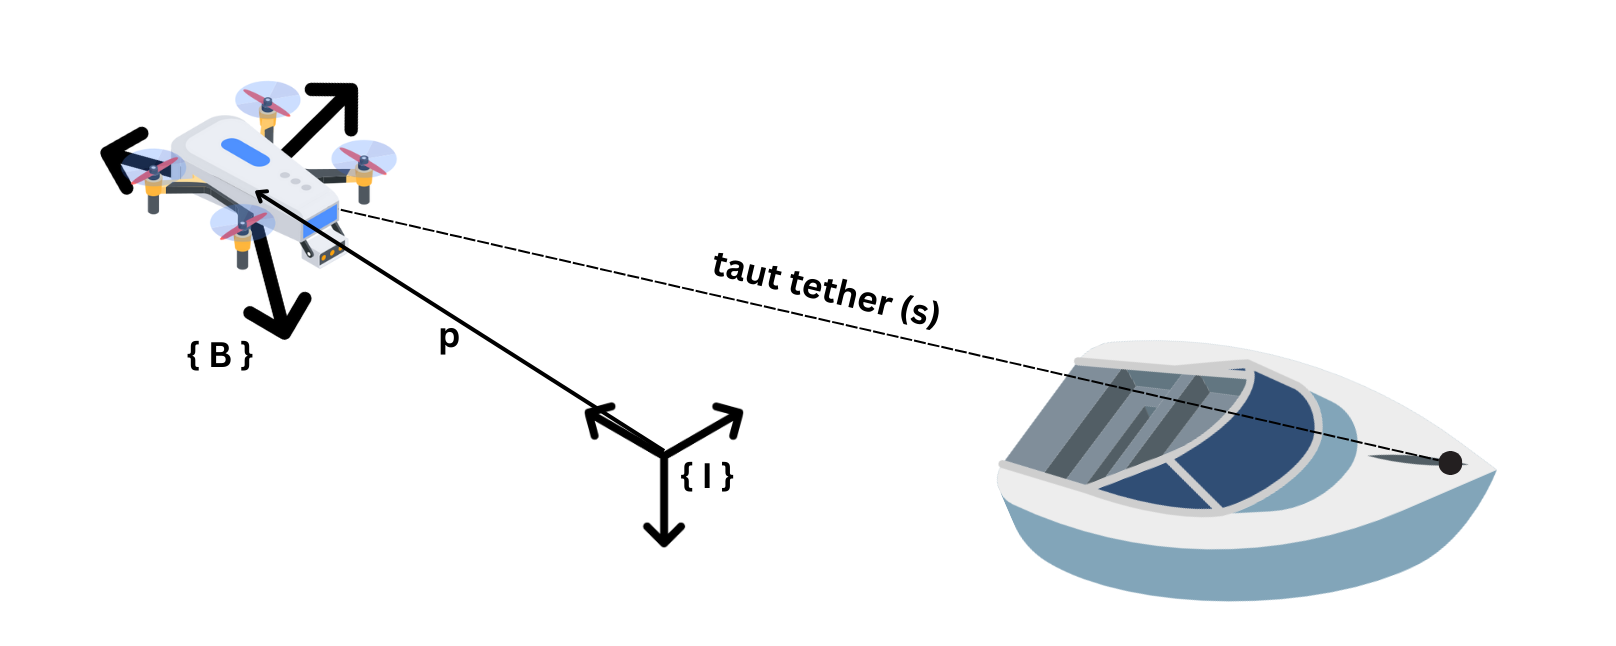
\includegraphics[width=0.8\textwidth]{Figures/background/frames.png}
    \caption{Inertial reference frame \(\{\mathcal{I}\}\) and body-fixed reference frame \(\{\mathcal{B}\}\) attached to the \gls{uav}, illustrating the position vector \(p\) and the relative orientation between frames.}
    \label{fig:reference_frames}
\end{figure}

\subsubsection{Rigid Body Kinematics}

The rigid-body kinematics describe how the position and orientation of the \gls{uav} evolve, relating the configuration variables \((p, R)\) to the linear and angular velocities expressed in the body-fixed frame. The time evolution of the position, expressed in the inertial frame, is given by
\begin{equation}
\dot{p} = R v ,
\end{equation}
where \(v \in \mathbb{R}^3\) denotes the linear velocity expressed in the body-fixed frame.

The time evolution of the orientation is described by
\begin{equation}
\dot{R} = R S(\omega),
\end{equation}
where \(\omega \in \mathbb{R}^3\) denotes the angular velocity expressed in the body-fixed frame, and \(S(\omega)\) is the associated skew-symmetric matrix defined as
\begin{equation}
S(\omega)=
\begin{bmatrix}
0 & -\omega_z & \omega_y \\
\omega_z & 0 & -\omega_x \\
-\omega_y & \omega_x & 0
\end{bmatrix}.
\end{equation}

\subsubsection{Rigid Body Dynamics}

The rigid-body dynamics describe how the linear and angular velocities of the \gls{uav} evolve under the influence of external forces and moments. These equations are expressed in the body-fixed frame using the Newton–Euler equations. Let \(m\) denote the \gls{uav} mass and \(J \in \mathbb{R}^{3 \times 3}\) its inertia matrix. The translational and rotational dynamics are given by
\begin{equation}
m \dot{v} = -S(\omega)\, m v + f,
\end{equation}
\begin{equation}
J \dot{\omega} = -S(\omega)\, J \omega + n,
\end{equation}
where \(f \in \mathbb{R}^3\) denotes the resultant external force and \(n \in \mathbb{R}^3\) the resultant external moment, both expressed in the body-fixed frame.

\subsubsection{Quadrotor UAV Input Forces and Moments}

The forces acting on the \gls{uav} include the thrust generated by the rotors, the gravitational force, and the force induced by the tether. While thrust and gravity are intrinsic to the vehicle, the tether introduces an additional coupling force that depends on the relative position between the \gls{uav} and its anchor point.

\paragraph{Thrust force and control moments}

The thrust is generated by the four rotors and acts along the body-fixed \(e_3\) axis, where \(e_3 = [0\;0\;1]^T\) denotes the unit vector aligned with the third axis of the body-fixed reference frame \(\{\mathcal{B}\}\), as shown in Fig.~\ref{fig:quadrotor_forces}. Each rotor produces an individual thrust \(T_i\), and the total thrust magnitude is given by

\begin{equation}
T = \sum_{i=1}^{4} T_i .
\end{equation}
The corresponding thrust force expressed in the body-fixed frame is
\begin{equation}
f_T = -T e_3 ,
\end{equation}

In addition to the total thrust, differential rotor speeds generate control moments about the body axes. These moments arise from asymmetric thrust distributions and rotor reaction torques, and are collected in the control moment vector
\begin{equation}
n = [n_x\; n_y\; n_z]^T .
\end{equation}

\begin{figure}[H]
    \centering
    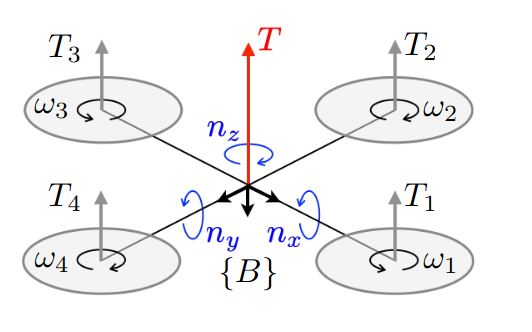
\includegraphics[width=0.35\textwidth]{Figures/background/forces.png}
    \caption{Body-fixed reference frame of the quadrotor showing the input forces and control moments generated by the rotors.}
    \label{fig:quadrotor_forces}
\end{figure}

\paragraph{Gravitational force}

The gravitational force acts along the vertical direction of the inertial frame. When expressed in the body-fixed frame, it is given by
\begin{equation}
f_g = m g R^{T} e_3 ,
\end{equation}
where \(m\) denotes the \gls{uav} mass and \(g\) the gravitational acceleration.


\paragraph{Tether-induced force}

The tether is modelled as a tension force acting along the line connecting the \gls{uav} to a fixed anchor point. Let \(p \in \mathbb{R}^3\) denote the \gls{uav} position and \(p_{\text{anchor}} \in \mathbb{R}^3\) the anchor point position, both expressed in the inertial frame. The relative position vector between the \gls{uav} and the tether anchor point is given by
\begin{equation}
s = p_{\text{anchor}} - p .
\end{equation}

The tether is assumed to remain taut at all times, such that its direction and magnitude are determined solely by the relative position between the \gls{uav} and the anchor point. Under this assumption, the tether is modelled as a straight line connecting the two points, and slack conditions are not considered. The regularised distance is defined as
\begin{equation}
\|s\|_\varepsilon = \sqrt{s^T s + \varepsilon^2}.
\end{equation}
The tether-induced force, expressed in the inertial frame, is defined as
\begin{equation}
F_{\text{tether}}(s) =
\left(T_0 + w_c\,\|s\|_\varepsilon\right)\frac{s}{\|s\|_\varepsilon},
\end{equation}
where \(T_0>0\) represents a minimum tension level that enforces continuous traction in the tether, \(w_c>0\) represents the effective weight of the cable per unit length, modelling the increase of required tension as the tether length grows, and \(\varepsilon>0\) is a small regularisation constant introduced to avoid numerical singularities when the relative distance becomes small.

This formulation is intended as a control-oriented approximation rather than a detailed structural model of a physical cable. The distance-dependent term reflects the intuitive effect that longer tethers require larger forces to remain taut due to the increasing weight of the cable.

When included in the \gls{uav} dynamics, the tether force is transformed to the body-fixed frame through the attitude rotation matrix and denoted by
\begin{equation}
f_{\text{tether}} = R^T F_{\text{tether}}.
\end{equation}


\paragraph{Resultant external force}

The resultant external force acting on the \gls{uav}, expressed in the body-fixed frame \(\{\mathcal{B}\}\), is given by
\begin{equation}
f = f_T + f_g + f_{\text{tether}} .
\end{equation}

\begin{figure}[H]
    \centering
    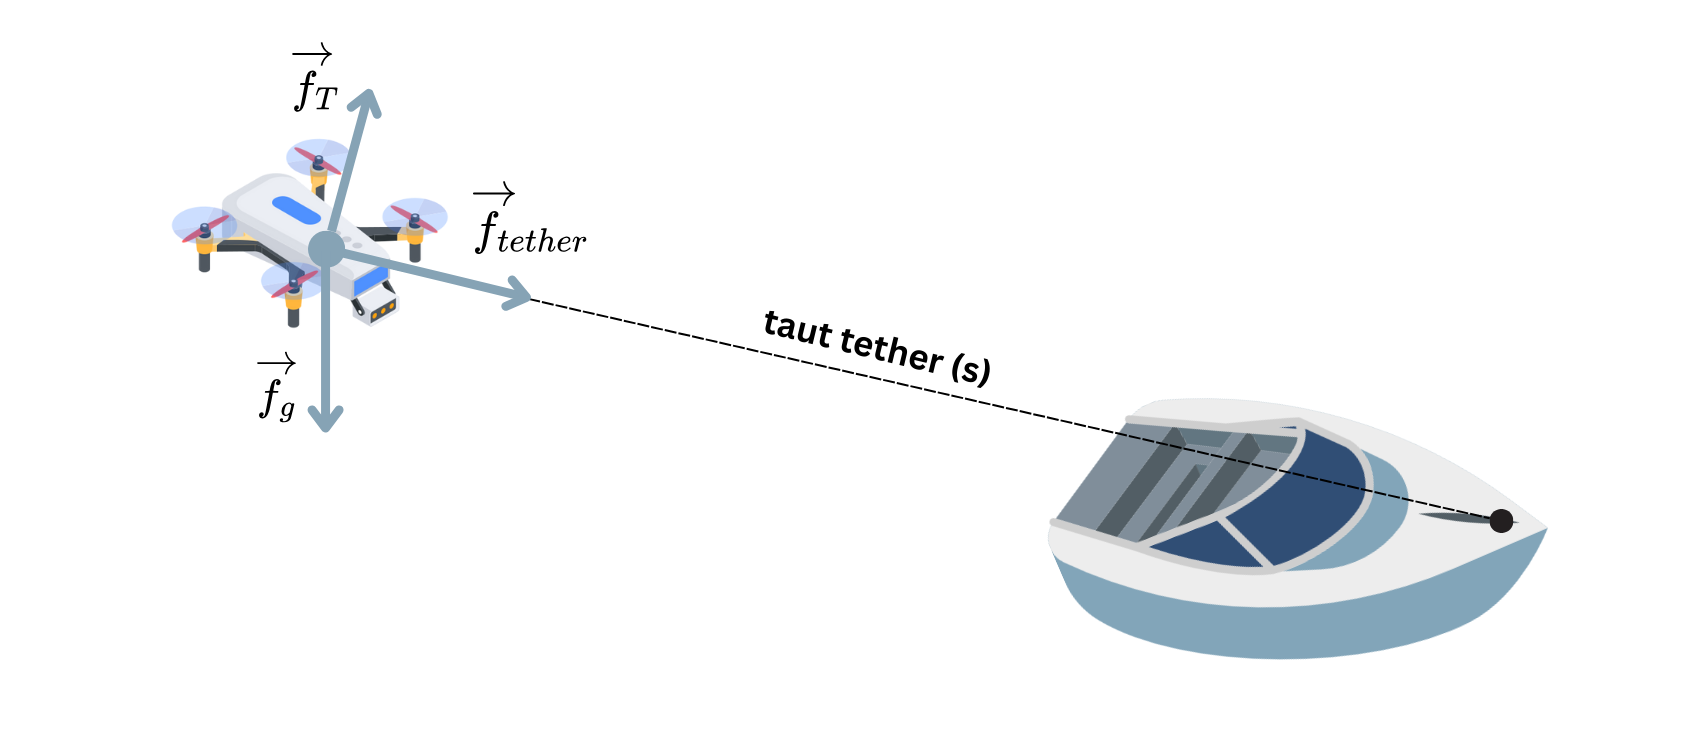
\includegraphics[width=0.8\textwidth]{Figures/background/all_forces.png}
    \caption{Forces acting on the tethered \gls{uav}: thrust \(\vec{f}_T\) generated by the rotors, gravitational force \(\vec{f}_g\), and tether tension \(\vec{f}_{\text{tether}}\). All forces are expressed in the body-fixed frame \(\{\mathcal{B}\}\).}
    \label{fig:uav_forces}
\end{figure}


\subsubsection{Complete UAV Model}

The complete dynamic model of the \gls{uav} is expressed in the body-fixed frame as
\begin{equation}
\begin{cases}
\dot{p} = R v, \\[6pt]
\dot{R} = R S(\omega), \\[6pt]
m \dot{v} =
- S(\omega)\, m v
- T e_3
+ m g R^{T} e_3
+ f_{\text{tether}}, \\[10pt]
J \dot{\omega} =
- S(\omega)\, J \omega
+ n,
\end{cases}
\end{equation}
where all forces are expressed in the body-fixed frame \(\{\mathcal{B}\}\).

The translational dynamics can be equivalently expressed in the inertial reference frame by differentiating \(\dot{p} = R v\), yielding
\begin{equation}
m \ddot{p} = -T R e_3 + m g e_3 + F_{\text{tether}},
\label{eq:inertial_dynamics}
\end{equation}
where \(F_{\text{tether}} = R f_{\text{tether}}\) denotes the tether force expressed in the inertial frame.



%%%%%%%%%%%%%%%%%%%%%%%%%%%%%%%%%%%%%%%%%%%%%%%%%%%%%%%%%%%%%%%%%%%%%%%%%

% MPC Formulation

%%%%%%%%%%%%%%%%%%%%%%%%%%%%%%%%%%%%%%%%%%%%%%%%%%%%%%%%%%%%%%%%%%%%%%%%%




\section{Motion Control}
\label{sec:theoretical_model_2}

\subsection{Control Architectures and Framework}
\label{subsec:control_methodology}

The motion control problem of the \gls{uav}–\gls{usv} system can be structured according to different architectures, depending on how coordination and control authority are distributed among agents \citep{olfati-saberConsensusCooperationNetworked2007,renDistributedConsensusMultiVehicle2010}. In a \emph{distributed} architecture, each agent has its own controller, and cooperation arises through information exchange or consensus-based mechanisms. In a \emph{centralised} formulation, the coupled system is treated as a single control entity, integrating all agent dynamics and constraints into one global optimisation problem.

Distributed control is computationally efficient and scalable, particularly when agent interactions are weak or communication delays are significant. These schemes rely on local control laws that use shared state information to achieve cooperative objectives such as formation keeping or consensus \citep{caoOverviewRecentProgress2013,olfati-saberConsensusCooperationNetworked2007}. However, in the tethered \gls{uav}–\gls{usv} configuration considered here, the physical connection introduces strong dynamic coupling and geometric constraints across the system. Under such conditions, distributed control requires additional coordination or constraint enforcement layers, which can lead to suboptimal behaviour.

A centralised control formulation provides a unified representation of the entire system, enabling direct handling of all interactions and constraints within a single optimisation problem \citep{zhangCooperativeControlFramework2025,novakCollaborativeObjectManipulation2024}. This global view allows control actions that inherently satisfy tether-related and dynamic coupling effects.

Within this framework, nonlinear model predictive control (\gls{nmpc}) is particularly suitable. \gls{nmpc} computes control inputs by repeatedly solving a finite-horizon optimal control problem that predicts the system’s evolution \citep{rawlingsModelPredictiveControl2020,gruneNonlinearModelPredictive2011}. This approach explicitly accounts for nonlinear dynamics, actuator limits, and coupling effects introduced by the tether. Although computationally demanding, \gls{nmpc} yields globally consistent and dynamically feasible control actions. Consequently, a centralised \gls{nmpc} strategy is adopted in this work as the foundation for the cooperative motion control framework.


\subsection{Model Predictive Control Principles}
\label{subsec:mpc_principles}

\gls{mpc} determines control actions not only from the current system state but also from predictions of its future evolution over a finite time horizon \citep{rawlingsModelPredictiveControl2020,camachoModelPredictiveControl2007}. By explicitly anticipating future behaviour, \gls{mpc} can handle system dynamics and constraints proactively rather than reactively.

At each control instant \(t\), the current state \(x(t)\) is measured and used as the initial condition for a prediction of length \(N\). Using a discrete-time model \(x_{k+1|t} = f(x_{k|t}, u_{k|t})\), the future states \(x_{k|t}\) are predicted for \(k = t, \dots, t+N\) based on a sequence of future control inputs \(u_{k|t}\) \citep{mayneConstrainedModelPredictive2000}. An optimisation problem is then solved to determine the control sequence that best achieves the desired objectives, such as trajectory tracking or regulation, while satisfying physical and operational constraints. Only the first input \(u_{t|t}\) is applied, and the process repeats at the next step, implementing the receding-horizon principle.

A key advantage of \gls{mpc} is its ability to handle constraints explicitly. Bounds on states and inputs, such as actuator limits, safety margins, or geometric restrictions, are directly incorporated into the optimisation problem \citep{gruneNonlinearModelPredictive2011}.

The general discrete-time formulation can be expressed as
\begin{equation}
\min_{u_{t|t},\dots,u_{t+N-1|t}}
\left[
\sum_{k=t}^{t+N-1} q(x_{k|t}, u_{k|t}) + p(x_{t+N|t})
\right],
\end{equation}
subject to
\begin{align}
x_{k+1|t} &= f(x_{k|t}, u_{k|t}), \quad k = t, \dots, t+N-1, \\
x_{t|t} &= x(t), \\
x_{k|t} &\in \mathcal{X}, \quad k = t+1, \dots, t+N, \\
u_{k|t} &\in \mathcal{U}, \quad k = t, \dots, t+N-1, \\
x_{t+N|t} &\in \mathcal{X}_f ,
\end{align}
where \(x_{k|t}\) and \(u_{k|t}\) denote the predicted state and input at step \(k\) given information at time \(t\). The function \(f(\cdot)\) represents the system dynamics, \(q(\cdot)\) is the stage cost, and \(p(\cdot)\) the terminal cost. The sets \(\mathcal{X}\), \(\mathcal{U}\), and \(\mathcal{X}_f\) define admissible states, inputs, and terminal conditions, respectively.

When \(f(\cdot)\) is nonlinear, the resulting \gls{nmpc} formulation allows the controller to directly account for nonlinear dynamics and coupling effects, which are relevant in the tethered \gls{uav}–\gls{usv} system considered in this work. Although the detailed stability and recursive feasibility conditions of NMPC are not discussed here, they will be further explored and analysed in the dissertation.


\subsection{NMPC Formulation}
\subsubsection{Prediction Model}

The control problem is formulated at the translational level by assuming a hierarchical control structure, which is standard in \gls{nmpc} applications for aerial vehicles. The \gls{nmpc} regulates the translational motion of the \gls{uav}, while the attitude dynamics are handled by a lower-level controller operating at a higher frequency.

Under this assumption, the translational dynamics expressed in the inertial reference frame, given in \eqref{eq:inertial_dynamics}, are adopted as the basis for the prediction model. Dividing the inertial-frame dynamics by the vehicle mass and introducing a virtual control input corresponding to the acceleration generated by the thrust force, the translational dynamics used for prediction are written as
\begin{equation}
\ddot{p} = u_d + g e_3 + a_{\text{tether}},
\end{equation}
where
\begin{equation}
u_d = -\frac{T}{m} R e_3
\end{equation}
denotes the inertial acceleration generated by the thrust, and
\begin{equation}
a_{\text{tether}} = \frac{1}{m} F_{\text{tether}}
\end{equation}
represents the acceleration induced by the tether.


\subsubsection{State and Input Definition}

Based on the prediction model above, the state vector considered by the \gls{nmpc} is reduced to the translational state
\begin{equation}
x =
\begin{bmatrix}
p &
\dot{p}
\end{bmatrix}^T \in \mathbb{R}^6,
\end{equation}
while the control input is given by the virtual acceleration
\begin{equation}
u = u_d \in \mathbb{R}^3.
\end{equation}


\subsubsection{NMPC Cost Function}

The \gls{nmpc} cost function is designed to track a desired translational trajectory while penalising excessive control effort. Over a prediction horizon of length \(N\), the cost function is defined as
\begin{equation}
J =
\sum_{k=1}^{N}
\Big[
(p_k - p_k^{\text{ref}})^T Q_p (p_k - p_k^{\text{ref}})
+
(\dot{p}_k - \dot{p}_k^{\text{ref}})^T Q_{\dot{p}} (\dot{p}_k - \dot{p}_k^{\text{ref}})
\Big]
+
\sum_{k=0}^{N-1}
u_k^T R u_k,
\end{equation}
where \(Q_p\), \(Q_{\dot{p}}\), and \(R\) are positive definite weighting matrices that balance trajectory tracking accuracy and control effort.

The \gls{nmpc} formulation also accounts for state and input constraints arising from physical, safety, and operational limitations of the tethered \gls{uav}. The explicit definition of these constraints is provided in Chapter~\ref{chapter:implementation}.
